\documentclass[sigsmall]{acmart}

\usepackage{graphicx}

\title{Summary of \emph{How Effective Are Commonly-Used Ad-Blockers?}}
\author{Matthew Oros, Sonny Smith, Michael Terekhov, Dennis Ulichney}

\setcopyright{none}
\settopmatter{printacmref=false}

\begin{document}
\maketitle


\section*{Abstract}
With the development of the internet web pages, online advertisements have also developed. Online advertisements can help find products that a user has been looking for, but they often ruin user experiences. Online advertisements might take up the whole space of a web page, and for mobile users, online advertisements might even make the usage of the page impossible. This research focuses on the software that removes such advertisements from web pages. The research paper includes an introduction, breakdown/related work, experiment design, results, and conclusion/future work.  \cite{}

\section*{Introduction}
The services offered online are mostly free and the most common way to monetize them is through online advertising. Online ads can be helpful, but most users find them to be one of the most annoying things on the internet. Most internet users want to minimize the number of ads they see and various ad-blocking software can be used to achieve this. The easiest and most popular way to block ads is to use browser extensions. An advanced ad-blocking method is to use specialized software that blocks incoming ad domains. Advanced software is considered more reliable, which means it blocks more ads. The purpose of this study is to find out how effective ad-blocking extensions are. This study focuses on the most popular browser ad blockers and their effectiveness compared to Pi-Hole software (the advanced software used for this study). Ad-blocking extensions that were utilized are AdBlock Plus, AdBlock, uBlock Origin, Privacy Badger, and Ghostery. Internet browsers that were utilized to test the software are Chrome, Microsoft Edge, and Firefox.


\section*{Background/Related Work}


\section*{Experiment Design}

\section*{Results}

test

\begin{figure}
  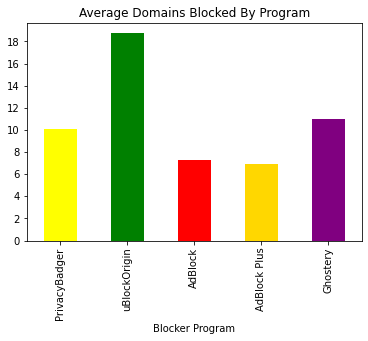
\includegraphics[width=\linewidth]{AvgByProgram.png}
  \caption{This graph compares the average number of domains detected and blocked by each blocking software.}
  \label{fig:graph1}
\end{figure}

test2

\begin{figure}
  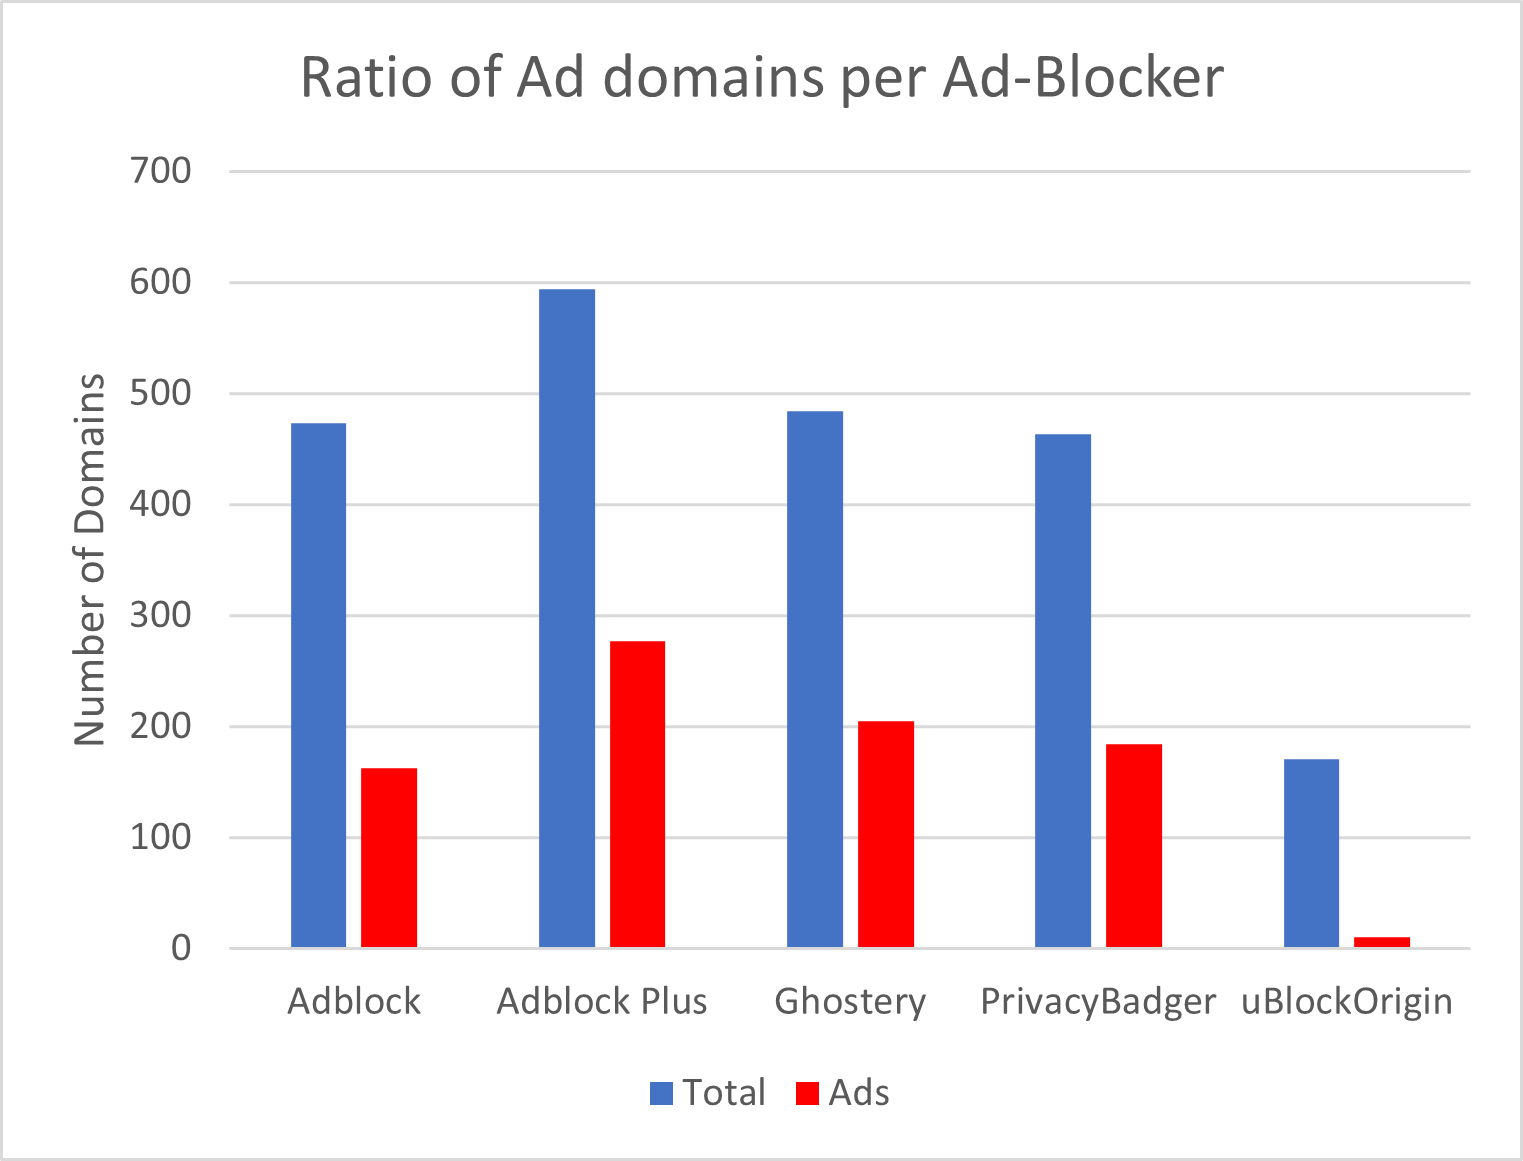
\includegraphics[scale =1.5]{Ratio-of-Ad-domains-per-ad-blocker.png}
  \caption{The total domains encountered by each blocker compared to the proportion of ads from those domains.}
  \label{fig:graph2}
\end{figure}

test3


\section*{Conclusion/Future Work}


\bibliographystyle{acm}
\bibliography{myBib}
\end{document}